\documentclass[a4paper,12pt]{report}
\usepackage[T1]{fontenc}
\usepackage[utf8]{inputenc}
\usepackage[italian]{babel}
\usepackage{graphicx}
\usepackage{listings}
\usepackage{color}
\usepackage[debug,pdftitle={Relazione},
bookmarks=true,colorlinks=true,urlcolor=magenta,
linkcolor=black,pagebackref=true,hyperindex=true]{hyperref}

\usepackage{geometry} %for the margins



\definecolor{dkgreen}{rgb}{0,0.6,0}
\definecolor{gray}{rgb}{0.5,0.5,0.5}
\definecolor{mauve}{rgb}{0.58,0,0.82}

\lstset{frame=tb,
  language=Java,
  aboveskip=3mm,
  belowskip=3mm,
  showstringspaces=false,
  columns=flexible,
  basicstyle={\small\ttfamily},
  numbers=none,
  numberstyle=\tiny\color{gray},
  keywordstyle=\color{blue},
  commentstyle=\color{dkgreen},
  stringstyle=\color{mauve},
  breaklines=true,
  breakatwhitespace=true,
  tabsize=3
}


\begin{document}


\title{Simulazione per trasporto di merci su gomma su scala regionale }\author{Davide Agostini}\date{Anno 2020/2021}

\begin{titlepage}
\newgeometry{left=1cm,right=1cm,top=3cm,bottom=3.5cm}  %specific margins for this page

\begin{center}

{\huge POLITECNICO DI TORINO}\\[1.5cm]
\textbf{Corso di Laurea in Ingeneria Gestionale\\Classe L-8 Ingegneria dell’informazione}\\[1.5cm]
%\textbf{Corso di Laurea Magistrale\\in Ingegneria Matematica}\\[3cm]

{\Large Tesi di Laurea Triennale}\\[1cm]
%{\Large Tesi di Laurea Magistrale}\\[0.5cm]
\textbf{\LARGE Simulazione per trasporto di merci su gomma su scala regionale}\\[1cm]

\includegraphics[width=0.4\textwidth]{./Images/logo.jpg}
\vspace{3cm}


\begin{minipage}{0.85\textwidth}
\begin{flushleft}\large
\textbf{Relatore} \hfill \textbf{Candidato}\\
prof. Fulvio Corno \hfill Davide Agostini\\
\end{flushleft}
\end{minipage}

\vspace{\fill}

Anno Accademico 2020-2021
\end{center}

\restoregeometry %restor default margins 

\end{titlepage}

\clearpage
\null
\thispagestyle{empty}
\clearpage

\tableofcontents

\clearpage
\null
\thispagestyle{empty}
\clearpage

\chapter*{Proposta dello studente}
\section*{Studente proponente}
s263632 Agostini Davide
\section*{Titolo della proposta}
Simulazione per trasporto di merci su gomma su scala regionale
\section*{Descrizione del problema proposto}
Nell’era dell’economia digitale l’e-Commerce si è affermata dapprima con grandi colossi internazionali e successivamente anche nelle piccole aziende locali, con effetti importanti sulla logistica applicata ai trasporti su gomma, su binari o tramite aereo.
Il problema presenta molteplici realtà, difatti sono tantissimi gli aspetti che la logistica stessa deve affrontare, dalla gestione dei magazzini alle consegne in città.\\
Tale applicazione si sofferma solo su determinati aspetti dell'argomento, in particolar modo i trasporti su gomma da magazzino a città e tralascia ciò che riguarda la gestione dei dipendenti e quella del magazzino.
\section*{Descrizione della rilevanza gestionale del problema}
Il problema logistico del trasporto viene spiegato e studiato in diversi casi in quanto variando i vincoli considerati si possono ottenere soluzioni molto diverse tra loro.\\
Utilizzando data-set non specifici e non di singole aziende, permetto di creare un'applicazione simil-realistica con l'obiettivo di simulare l'andamento di una giornata di lavoro lasciando all'utente la scelta di diversi elementi.\\
Lo scopo di tale simulazione è dare modo ad una qualsiasi azienda di osservare come il cambiamento di poche variabili sia radicale per il soddisfacimento della domanda esterna.
\subsection*{Descrizione dei data-set per la valutazione}
Come dichiarato in precedenza i data-set utilizzati non appartengono ad una specifica azienda, ma sono basati sui comuni e sulla distanza tra essi.\\
E' importante evidenziare che il calcolo della distanza non viene basato solo su latitudine e longitudine, ma calcolato sulla base delle diverse strade in ogni regione.\\
In particolar modo è presente sui data-set il tempo reale impiegato da un mezzo che parte da un comune per raggiungerne un altro.\\
I dati presenti sono oltre il milione per ogni regione, ad esempio per la regione Piemonte il dataset offre oltre 8 milioni di dati.\\
Il data-set utilizzato sarà rielaborato in base alla regione scelta da utente.\\
\begin{itemize}
\item I data-set sui comuni sono disponibili sul sito Istat con il loro codice alfanumerico al \\link: \href{https://www.istat.it/storage/codici-unita-amministrative/Elenco-comuni-italiani.xls}{https://www.istat.it/storage/codici-unita-amministrative/Elenco-comuni-italiani.xls}.
\item I data-set sul reale minutaggio tra i comuni è presente in questo\\ link:
\href{https://www.istat.it/it/archivio/157423}{https://www.istat.it/it/archivio/157423}.
\end{itemize}
\subsection*{Descrizione preliminare degli algoritmi coinvolti}
L'applicazione consiste nella scelta di una tra le seguenti opzioni: simulazione e ricorsione.\\
In primo luogo verrà chiesto all'utente di dichiarare dei parametri che verranno poi utilizzati in entrambe le opzioni, ovvero: la Regione da considerare, il comune nel quale vi è il magazzino principale e il numero di consegne da effettuare (ovvero il numero di comuni nel quale deve essere effettuata la consegna).\\
Per semplicità il comune corrisponde alla consegna da effettuare e perciò non vi possono essere più consegne per ogni comune.\\
Successivamente verrà creato un grafo utilizzando i data-set della regione considerata.\\
In particolar modo si creerà un grafo a maglia completa aventi come nodi i comuni nel quale si deve effettuare la consegna e come archi il minutaggio che intercorre tra un comune ed un altro.\\
I comuni delle consegne sono scelti casualmente e il numero coincide con quello inserito precedentemente dall'utente.\\
Successivamente l'applicazione fornirà due possibilità:
\begin{itemize}
\item La prima è una simulazione dei percorsi effettuati dai veicoli.\\
Dopo aver scelto il numero di veicoli, il numero delle consegne massime per percorso e il minutaggio entro il quale si vuole tornare al magazzino, verrà data all'utente la possibilità di effettuare una simulazione Bilanciata o non Bilanciata.\\
\begin{description}
\item[Simulazione Bilanciata] Simulazione ad eventi discreti che riporta i tragitti effettuati.\\
Ogni veicolo parte dal magazzino al tempo zero ed effettua la consegna nel comune disponibile più vicino dal quale è stato effettuato l'ordine.\\
Dopo aver effettuato la consegna, per la successiva ogni veicolo calcola il comune più vicino e così via fino alla fine della giornata lavorativa o al raggiungimento del numero massimo di consegne.
\item[Simulazione non Bilanciata] Insieme di ricorsioni che trovano il percorso migliore di ogni veicolo date le variabili e i comuni già raggiunti, simulando il sistema dei mezzi.\\
Considerato il primo veicolo viene effettuata la ricorsione per trovare il percorso migliore.\\
Successivamente si passa al secondo veicolo al quale vengono tolti i comuni già raggiunti e così via.
\end{description}
\item La seconda permette all'utente di scegliere il minutaggio massimo ed il comune nel quale si vuole effettuare l'ultima consegna ed utilizza la ricorsione per trovare il percorso ottimo.\\
\end{itemize}
\subsection*{Descrizione preliminare delle funzionalità previste per l’applicazione software}
\begin{enumerate}
\item Per prima cosa verrà richiesto all'utente di scegliere la regione.
\item Si sbloccheranno poi: un menù a tendina con i comuni per scegliere il magazzino principale dal quale i veicoli partiranno ed un textfield che permette di inserire il numero di consegne da effettuare.
\item Dopo aver creato il grafo all'utente verranno presentate due opzioni: la prima sarà effettuare la simulazione, la seconda consisterà nell'ottimizzare un unico percorso.
\begin{itemize}
\item Nel caso della scelta della simulazione verrà chiesto all'utente di inserire: il numero di veicoli, il numero massimo di consegne che questi potranno effettuare, il tempo di durata della giornata nella simulazione e il tipo di simulazione (Bilanciata o non Bilanciata).\\
Come risultato viene mostrato il percorso dei veicoli, il numero di consegne effettuate ed il numero di consegne eventualmente non effettuate.
\item Nel caso di ottimizzazione del percorso viene richiesto all'utente la destinazione e il minutaggio massimo con il quale si vuole che il veicolo arrivi a destinazione.
\end{itemize}
\end{enumerate}


\chapter{Descrizione del problema affrontato}
\label{cap:Descrizione}
Uno degli obiettivi principali di ogni azienda di qualsiasi natura consiste nell'utilizzare al meglio le proprie risorse e successivamente di espandersi cercando di raggiungere più persone possibili
aumentando di conseguenza il profitto. \\
In un mondo in cui si vuole fare attenzione ai particolari, che talvolta sono state trascurati, è imperativo ottimizzare ogni singola processo per permettere una crescita sostenibile.\\
Per questo motivo al giorno d'oggi si ricorre a metodi come ad esempio l' industria 4.0 con l'obiettivo di migliorare la logistica dell' azienda.\\
Ma cosa è effettivamente la logistica?\\Secondo il Council of Supply Chain Management Professionals:
\begin{quote}
``{\em La gestione della logistica è quella parte della gestione della supply chain che pianifica, implementa e controlla l'efficienza e l'efficacia dei flussi in ingresso e in uscita e dello stoccaggio di merci, di servizi e di informazioni correlate tra il punto di origine e il punto di consumo al fine di soddisfare le esigenze dei clienti.}''
\end{quote}
Si nota come la logistica si occupi di ogni piccolo aspetto della vita del processo: dall'origine alla conclusione, ovvero dalla produzione alla distribuzione.\\
Per questa ragione, è possibile distinguere la logistica a seconda del processo di cui si occupa e di come si innesta nel percorso industriale.\\
In tale ambito si è dato spazio alla logistica distributiva o dei trasporti che si occupa della gestione della rete di distribuzione della merce, secondo gli accordi intercorsi fra l'azienda e il cliente.\\
L'applicazione creata si propone quindi di monitorare la consegna del prodotto su gomma ad un altro ente in un determinato periodo di tempo.\\
La realizzazione dell'applicazione è stata influenzata dai principali indicatori di performance per una logistica di qualità finalizzata a ottimizzare ogni processo.\\
Si parla quindi di:
\begin{itemize}
	\item Efficienza dei processi.
	\item Qualità delle infrastrutture relative al commercio e al trasporto.
	\item Capacità di rintracciare e seguire le spedizioni.
	\item Frequenza con la quale le spedizioni raggiungono i destinatari entro i tempi prestabiliti.
\end{itemize}
Utilizzando un data-set intra-regionale sulla distanza tra i vari comuni si è deciso di porre un magazzino principale che si occupa delle spedizioni solamente nella regione di origine.\\
Non viene quindi trattato il problema legato alla distanza di un comune in altre regioni e le altre verranno immediatamente non considerate al momento della scelta di quest'ultima.\\
Obiettivo dell'applicazione è essere strumento e non un fine in grado di indicare l'unica "ottima" soluzione, poichè in un problema così vasto cercare un soluzione ottima non considerando 
molte variabili può essere inutile e dispendioso.\\ Per questo motivo si è dato spazio alla simulazione: ovvero un' applicazione in grado di simulare l'evoluzione dei percorsi di ogni mezzo permettendo all'utente di osservare la soluzione ottimale a seconda delle risorse disponibili.\\
E' stata inoltre data all' utente la possibilità di scegliere se eseguire una simulazione di tipo bilanciato o non bilanciato il cui risultato è interpretabile diversamente a seconda dello scenario scelto.
\begin{description}
	\item[Simulazione bilanciata] Tutti i veicoli al momento dell'avvio della simulazione scelgono, se presente, una consegna da effettuare. 
	\item[Simulazione non bilanciata] Viene simulato il percorso migliore del primo veicolo e successivamente, tenendo conto del tragitto individuato, viene analizzato il secondo e così via.
\end{description}
E' stata inoltre aggiunta la possibilità di trovare il percorso ottimo di un singolo veicolo, utile nel caso in cui si voglia analizzare la differenza tra il tragitto ottenuto con la simulazione bilanciata e il miglior tragitto oppure nel caso in cui si utilizzino strumenti esterni all'azienda.\\
Le criticità del problema sono legate alla presenza di un limitato numero di variabili, in quanto ad esempio non vengono considerati magazzino, capacità delle risorse umane e del carburante per ogni veicolo.\\
Ciò che viene ottenuto tramite l' applicazione è uno strumento per permettere uno studio più dettagliato dello scenario considerato e richiede perciò di essere analizzato attivamente dall'utente.
\chapter{Descrizione del data-set utilizzato per l’analisi}
Per la realizzazione dell'applicazione sono state utilizzati due data-set forniti dall'Istat che contengono le informazioni riguardanti i comuni e la loro locazione.\\
Un data-set è composto da un' unica tabella denominata ``\texttt{nome\_comune}'' e contiene generalità sui diversi comuni
come ad esempio nome italiano comune, codice alfa-numerico e regione di appartenenza.\\
Per semplicità si è scelto di lavorare solamente con alcuni dati del data-set dell'Istat
per non affaticare la ricerca nell'applicazione.\\
Il secondo data-set è decisamente più corposo e offre per ogni regione le matrici 
origine-destinazione delle distanze in metri e dei tempi di percorrenza in minuti tra i comuni 
italiani.\\
Il minutaggio è stato calcolato attraverso strumenti GIS e utilizzando un grafo stradale 
commerciale, quindi rappresenta una struttura dati più possibile vicina alla realtà.\\
Nel data-set fornito dall'Istat il comune di origine è appartenente alla regione mentre
i comuni di destinazione non sono classificati per regione.\\
Ai fini dell'applicazione per ogni tabella della regione è stata effettuata una parziale rielaborazione
dei dati, cercando di eliminare i comuni non appartenenti alla area considerata.\\
Non è stata possibile una completa compilazione delle tabelle con comuni origine e destinazione
attinenti unicamente alla regione considerata poiché la distribuzione dei codici comunali è
talvolta incongruente.\\
Per tali motivi esistono tabelle con più righe rispetto a quelle effettive.\\
Solamente per Piemonte (Origine qualunque e Destinazione Piemonte), Sicilia e Sardegna è stato
fatta una rielaborazione diversa.\\
Tale data-set è stato inoltre redatto nel 2013 perciò sono presenti comuni che sono stati dismessi 
nel corso degli anni.
\begin{figure}[h]
\begin{center}
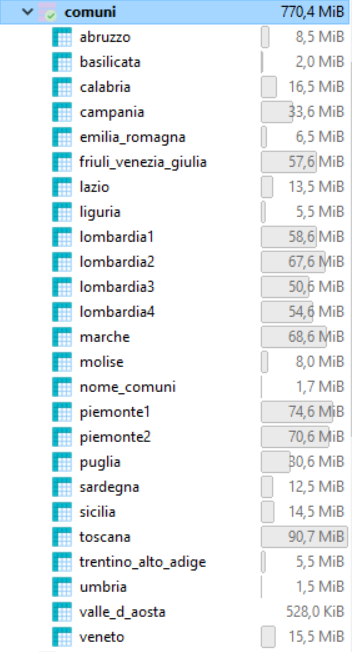
\includegraphics[width=0.3\textwidth]{Images/DB.png} 
\caption{Data-set completo}
\end{center}
\end{figure}


\subsection{Tabella nome\_comune}
Composta da 7904 elementi, contiene tutti i comuni italiani e le loro generalità.\\
La tabella ha come chiave primaria ``\texttt{codice\_comune}'' che rappresenta il codice alfanumerico
univoco di ogni comune dichiarato in Stringa di caratteri.\\
La colonna ``\texttt{codice\_int}'' invece rappresenta il codice alfanumerico del comune espresso in numeri.\\
``\texttt{codice\_regione}'' e ``\texttt{nome\_regione}'' sono rispettivamente l'identificativo della regione
e il suo nome completo.\\
Intuitivamente ``\texttt{nome\_comune}'' è il nome italiano del comune considerato (ai fini dell'applicazione
è stato tralasciato il nome in lingua non italiana).
\begin{figure}[h]
\begin{center}
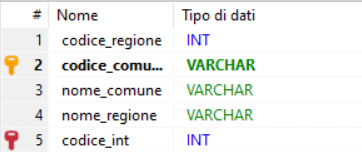
\includegraphics[width=0.4\textwidth]{Images/tabellaNomeComune.png}
\caption{Tabella nome\_comune}  
\end{center}
\end{figure}

\subsection{Tabella di una Regione}
Le tabelle con il nome della regione sono tabelle appartenenti al secondo data-set e contengono le
stesse informazioni suddivise per regione.\\
La chiave primaria è composta dalle colonne ``\texttt{comune\_partenza}'' e ``\texttt{comune\_arrivo}'' ovvero la coppia 
``\texttt{comune\_partenza}'' e ``\texttt{comune\_arrivo}'' è univoca.\\
Le due colonne rappresentano il codice alfanumerico del comune e sono di tipologia Interi  poichè permettono all'applicazione una più veloce lettura dei dati rispetto alle stringhe.\\
Sono quindi chiave esterna di ``\texttt{codice\_int}'' della tabella ``\texttt{nome\_comune}'', ma non è stato
possibile evidenziare questa relazione tramite i software utilizzati  in quanto sono presenti anche comuni depennati
dopo il 2013 (La foreign key richiede che per ogni elemento di tale tabella esista un elemento
della tabella al quale si vuole legare e in ``\texttt{nome\_comuni}'' i comuni depennati del 2021 non esistono).
\begin{figure}[h]
\begin{center}
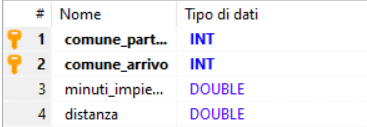
\includegraphics[width=0.4\textwidth]{Images/tabellaRegione.png} 
\caption{Tabella di una qualsiasi regione}  
\end{center}
\end{figure}

\subsection{Tabelle Piemonte1, Piemonte2, Lombardia1, Lombardia2, Lombardia3 e Lombardia4}
Le tabelle sopra citate sono state divise per la loro lunghezza nel data-set dell'Istat e 
rappresentano le regioni di Piemonte e Lombardia.\\
La suddivisione è avvenuta in modo tale che le tabelle fossero complementari tra di loro, ovvero
tuple presenti su una non sono presenti nell'altra.\\
E' stato successivamente utilizzato l'operatore \textbf{UNION} nella Query Sql per sopperire a questo svantaggio.\\
Rispetto alle altre regioni necessitano quindi una Query Sql diversa, ma non richiedono ulteriori attenzioni all'interno dell'applicazione.

\chapter{Descrizione Strutture dati ed algoritmi}
\label{Cap:DescrizioneStrutture}
\section{Strutture dati utilizzate}
L'applicazione, sviluppata in linguaggio java, segue il pattern MVC (Model-View-Controller) ed il pattern
DAO (Data-Access-Object) per far si' che all'interno dello sviluppo dell'applicazione si tengano
separati l'accesso ai dati del database, la parte algoritmica del programma e l'interfaccia utente.\\
Sono quindi presenti tre packages con ognuno una proprietà appena descritta:

\subsection{it.polito.tdp.SimulazioneTrasporti}
Il package ha come obiettivo quello di essere l'interfaccia per l'utente e per fare ciò contiene
il \texttt{Main}, l'\texttt{FXML Controller} e l'\texttt{EntryPoint}.
\begin{description}
	\item[\texttt{Main}] necessario per l'avvio dell'applicazione stessa.
	\item[\texttt{EntryPoint}] gestisce avvio interfaccia nel quale verranno inseriti i dati necessari.
	\item[\texttt{FXMLController}] Riceve dati in Input e collega l'interfaccia con il Model (logica dell'applicazione)
	ed è quindi la classe che interpreta i dati inseriti da utente e dopo un primo controllo permette 
	lo svolgimento degli algoritmi fondamentali.
\end{description}

\subsection{it.polito.tdp.SimulazioneTrasporti.db}
Fulcro attraverso il quale l'applicazione prende i dati necessari dal database ed esegue una parziale 
scrematura delle informazioni che poi andranno al \texttt{Model} tramite delle query SQL.\\
E' formato dalle classi \texttt{DBConnect} e \texttt{TrasportiDao}.
\begin{description}
	\item[\texttt{DBConnect}] Connessione con database.
	\item[\texttt{TrasportiDao}] Riceve come Input richieste dal Model e attraverso query SQL consegna i dati voluti.
\end{description}

\subsection{it.polito.tdp.SimulazioneTrasporti.model}
Package che contiene la logica applicativa dell'applicazione e attraverso la classe Model svolge la maggior parte delle operazioni.\\
Contiene ben 8 classi: \texttt{Collegamento, Comuni, Consegna, Event, Model, Regione, Simulator, Veicolo}.\\
\begin{description}
	\item[\texttt{Collegamento}] Classe che permette la creazione degli archi nel grafo iniziale.
	\item[\texttt{Comuni} e \texttt{Regione}] classi che identificano comuni e regioni con attributivi necessari.
	\item[\texttt{Consegna}] classe che associa un comune a un tempo ed è principalmente utilizzato per descrivere una consegna.
	\item[\texttt{Simulator} e \texttt{Event}] Classi attraverso il quale avviene la Simulazione bilanciata.
	\item[\texttt{Veicolo}]  classe che identifica il veicolo e in particolar modo permette di ottenere l percorso tramite una \texttt{List<Consegna>}, ovvero tramite una lista di consegne effettuate.
	\item[\texttt{Model}] Classe che collega ogni elemento dell'applicazione e si interfaccia sia con il package View e sia con il package Controller. Contiene inoltre la Ricorsione ovvero la logica per l'ottimizzazione del singolo percorso e della simulazione non bilanciata.
\end{description}

\section{Descrizione algoritmi utilizzati}
\label{Sec:Algoritmi}
L'applicazione è divisa in tre fasi principali all'interno del quale viene chiesto all'utente di
inserire vincoli fondamentali e necessari allo svolgimento degli algoritmi più importanti.\\
La prima fase coincide con la scelta della regione e nonostante sia la più corta corrisponde alla
scelta della tabella dal quale prendere i comuni desiderati.\\
La seconda fase è la creazione di un grafo e richiede una scelta di un magazzino principale e di
un numero di ordini che corrisponderanno poi ai comuni nel quale si vuole effettuare la consegna.\\
La terza fase è a sua volta suddivisa in Simulazione e Ottimizzazione:
\begin{itemize}
	\item La Simulazione richiede un numero di veicoli, un numero massimo di consegne, i minuti nel quale 
si vuole lavorare e la scelta della tipologia di bilanciamento.
	\item L'Ottimizzazione del singolo percorso corrisponde agli algoritmi di ricorsione e permette all'utente di scegliere la destinazione desiderata tra i comuni presi casualmente durante la creazione del grafo e un minutaggio entro il quale si vuole lavorare.
\end{itemize}
Per permettere lo svolgimento dell'applicazione sono state fatte delle semplificazioni che è necessario menzionare:
\begin{itemize}
	\item I veicoli nella simulazione alla partenza saranno a pieno pieno carico, ovvero non avranno bisogno di ritornare a magazzino per ricevere ulteriore merce.
	\item In un comune vi può essere un unico ordine e perciò il numero di consegne nella fase 2 corrisponde al numero di comuni nel grafo.
	\item Il veicolo una volta raggiunto il comune compie immediatamente la consegna e non viene considerato tempo aggiuntivo.
	\item Nella simulazione il numero massimo di consegne è espresso in Interi poichè si vuole che l'applicazione sia più generica possibile e non vincolata da Kg o litri.
	\item Il minutaggio impiegato per raggiungere il comune 'b' dal comune 'a' è lo stesso impiegato per  per raggiungere il comune
'a' dal comune 'b' (raramente il data-set non presenta entrambi i dati).
\end{itemize}
Si ricorda che è stata creata come uno strumento per una qualsiasi azienda per simulare l'andamento di una giornata lavorativa, perciò richiede che i dati successivamente ottenuti siano analizzati e studiati
al fine di migliorare le proprie capacità.

\subsection{Fase 1: Scelta della regione}
Corrisponde, come precedentemente accennato, alla fase più corta e si articola in tre semplici metodi
appartenenti a \texttt{TrasportiDao}, \texttt{Model} e \texttt{FXMLController}.
\begin{itemize}
	\item Nel metodo del \texttt{TrasportiDao} \texttt{listaRegioni()} viene restituita un'ArrayList di regioni italiane.
	\item Il metodo del \texttt{Model} \texttt{regioni()} (Listing~\ref{lst:regioni}) utilizza il metodo del \texttt{trasportiDao} per ottenere la lista e successivamente
esegue un \texttt{Collections.sort()} per ordinarle in ordine di nome (la classe regione implementa \texttt{Comparable(Regione)}).
	\item L'\texttt{FXMLController} per prima cosa popola la combo box \texttt{boxRegione} all'avvio dell'interfaccia
e poi utilizza il metodo \texttt{doRegione()} per effettuare i controlli necessari su ciò che è stato inserito
dall'utente.
\end{itemize}
Viene inoltre sbloccata la fase due e popolata la combo box \texttt{boxMagazzino} con i comuni della regione.
\begin{center}
\begin{lstlisting}[caption={Metodo di inserimento regione del Model},  label={lst:regioni},captionpos=b, language=Java]
	public List<Regione> regioni() {
		List<Regione> lista=new ArrayList<Regione>(dao.listaRegioni());
		Collections.sort(lista);
		return lista;
	}
\end{lstlisting}
\end{center}

\subsection{Fase 2: Simulazione degli ordini con creazione grafo}
L'utente sceglie il magazzino dal quale si vogliono far partire gli ordini nella combo box \texttt{boxMagazzino} e sceglie il numero di comuni che vuole raggiungere che coincide con il numero di ordini effettuati.\\
Per spiegare il funzionamento di questa fase si preferisce partire dal cervello dell'applicazione, cioè il \texttt{Model}.\\
Il grafo utilizzato corrisponde ad un \texttt{DefaultWeightedEdge} ovvero un grafo non direzionato e pesato avente
avente come vertici i comuni degli ordini e come archi il minutaggio impiegato tra questi.\\
Nel metodo del model \texttt{creaGrafo()} (Listing~\ref{lst:creaGrafo}) \footnote{Per rendere più compatto il codice, il metodo sotto riportato mostra solo il caso della regione Liguria} viene creata \texttt{listaComuniNo}, una ArrayList utilizzata nell'aggiunta
dei vertici del grafo.\\
In primo luogo vengono aggiunti tutti i comuni della regione, viene poi tolto il magazzino dalla lista e infine viene scelto casualmente un comune da aggiungere al grafo e da rimuovere dalla  lista (si evita così che il comune venga preso due volte).\\
Si passa poi all'aggiunta degli archi e con l'utilizzo di uno \texttt{switch} viene scelta la regione dal quale verranno prese le distanze e collegati i due comuni.\\
Scelta la regione per ogni comune-vertice del grafo verrà creata una\\ \texttt{HashMap<Integer,Collegamento>}
contenente come chiave il comune di arrivo e come come oggetto un elemento della classe Collegamento.\\
La classe collegamento appositamente creata contiene il comune di partenza, il comune di arrivo 
e il minutaggio impiegato per percorrere la distanza tra i due.
Il metodo utilizzato per popolare l'HashMap è in \texttt{TrasportiDao} e con una query SQL riceve come
Input un comune e riporta come Output tutti i collegamenti di quest'ultimo.\\
Con l'aiuto dell'HashMap viene controllata la presenza del collegamento e se non già presente nel
grafo, viene aggiunto l'arco.\\
Il grafo necessita di essere a maglia completa per far avvenire le operazioni successive, ovvero
richiede che tutti i vertici siano collegati tra di loro e perciò vi è la necessità di
svolgere un meccanismo apposito di controllo.\\
Nel caso in cui il numero di archi sia diverso dal numero di archi per un grafo completo allora verrà aggiunto 1 al contatore \texttt{n} e il metodo richiamerà se stesso.\\
La formula di controllo del numero di archi è:
\begin{equation}
\label{eq:equazione1}
\frac{N\cdot(N-1)}{2}
\end{equation}
dove N è il numero di vertici del grafo.\\
Nel caso in cui il contatore sia maggiore di 5, ovvero siano stati effettuati più di 5 tentativi
di creazione del grafo vi sarà un exception.\\
L'\texttt{FXMLController} ha il compito di controllare i dati in Input inseriti dall'utente e di richiamare 
il metodo \texttt{creaGrafo()} del \texttt{Model}.\\
Dopo aver ricevuto il grafo dal model, popola le cpmbo box \texttt{boxDestinazione} e la \texttt{txtComuni} con la lista dei
comuni nel grafo e infine sblocca la fase 3.\\

\begin{center}
\begin{lstlisting}[caption={Metodo del model creaGrafo() per la creazione del grafo}, label={lst:creaGrafo}, captionpos=b, language=Java]
public Graph<Comuni,DefaultWeightedEdge> creaGrafo(Regione regione,int numeroConsegne,Comuni magazzino ) throws Exception {
		if(n>5) {
			throw new Exception("Troppi tentativi");
		}
		this.magazzino=magazzino;
		grafo=new SimpleWeightedGraph<Comuni,DefaultWeightedEdge>(DefaultWeightedEdge.class);	
		ArrayList<Comuni> listaComuniNo=new ArrayList<Comuni>(listaComuni);
		
//		Aggiungo vertici
		grafo.addVertex(magazzino);
		listaComuniNo.remove(magazzino);
		for(int i=0;i<numeroConsegne;i++) {
			int casuale=(int) (Math.random()*listaComuniNo.size());
			Comuni vertice= listaComuniNo.get(casuale);
			listaComuniNo.remove(vertice);
			grafo.addVertex(vertice);
		}
		
//		Aggiungo archi
		switch(regione.getNomeRegione()) {
		case "Liguria":
			for(Comuni c:grafo.vertexSet()) {
			Map<Integer,Collegamento> mappaColl=new HashMap<Integer,Collegamento>	(dao.mappaCollegamentiLiguria(c.getCodiceInteroComune()));
				for(Comuni dest:grafo.vertexSet()) {
					if(!c.equals(dest) && !grafo.containsEdge(c, dest)) {
						int var=dest.getCodiceInteroComune();
						if(mappaColl.containsKey(var)) {
							Graphs.addEdge(grafo, c, dest, mappaColl.get(var).getPeso());
						} 
					}
				}
			};
			break;
		}
		
		int numArchi=(int) ( (numeroConsegne * (numeroConsegne+1) )/2);
		if(grafo.edgeSet().size()!=numArchi) {
			n++;
			this.creaGrafo(regione, numeroConsegne, magazzino);
		}
			
		return grafo;
			
		
}
	
\end{lstlisting}
\end{center}

\subsection{Fase 3: Simulazione e Ottimizzazione}
La Simulazione viene inizializzata nella classe \texttt{Model} e viene proseguita nella classe \texttt{Simulator},
mentre l'ottimizzazione viene direttamente implementata nei metodi \texttt{percorsoMigliore()} e \texttt{trovaRicorsivo()}
del \texttt{Model}.
\subsubsection{Simulazione}
In input vengono inseriti tramite textArea il numero dei veicoli, il numero massimo di consegne da effettuare per veicolo e
i minuti della giornata lavorativa e vengono convalidati dal metodo \texttt{doSimulazione()} dell' \texttt{FXMLController}.\\
Obiettivo della simulazione è trovare un percorso ad ogni veicolo utilizzato e sfruttare tutte
le risorse disponibili. \\
Per scegliere il tipo di simulazione da effettuare viene inserito un radio button che chiede
all'utente se effettuare una simulazione bilanciata o non bilanciata.
\subsubsection{Simulazione bilanciata}
Dopo aver scelto i numeri necessari per effettuare la simulazione l'applicazione bilancia il lavoro su tutti i veicoli preferendo un utilizzo più vasto rispetto ad uno migliore.\\
Ciò significa che non viene effettuata un ottimizzazione del percorso di ogni veicolo, ma una simulazione dell'andamento di una qualsiasi giornata per osservare gli effetti dello scenario considerato.\\
Anche una piccola variazione di un dato in input può provocare molte differenze di output.\\
Per la Simulazione bilanciata è stato preferito utilizzare un algoritmo che permette ai veicoli di osservare solo il
passo successivo, considerando perciò immutabili i passi precedenti.\\
Il veicolo, avendo a disposizione tutti gli archi del grafo, ricerca il comune più veloce da raggiungere
al quale si deve effettuare la consegna e nel caso in cui non sia in contraddizione con
i vincoli posti dall'utente e il comune non sia stato già raggiunto, viene effettuata la consegna.\\
Tale algoritmo garantisce ad ogni veicolo di tornare al magazzino in un tempo pressochè simile e 
non permettere grandi variazioni sugli orari lavorativi dei diversi veicoli.\\
La simulazione ad eventi discreti per essere operativa necessita di una classe \texttt{Event} che contiene
gli eventi fondamentali con i loro attributi ed una queue contenente i suddetti eventi.\\
In questo caso la classe \texttt{Event} contiene tre diversi tipologie di evento: \texttt{CONSEGNA\_EFFETTUATA, CONSEGNA\_IN\_CORSO, RITORNO\_MAGAZZINO} ed è caratterizzata da un veicolo, un comune ed il tempo
che serve a dare dinamicità alla simulazione (a seconda del tempo assume un ruolo nella queue).\\
Per permettere all'applicazione di effettuare la simulazione vi è bisogno di una inizializzazione
e un' elaborazione dei vari eventi.\\
\begin{itemize}
	\item Inizializzazione (metodo \texttt{init() Simulator}, Listing~\ref{lst:init}): inizializza i vari veicoli aggiungendo una
lista di consegne per ogni veicolo e inserisce nella queue l'evento \texttt{CONSEGNA\_IN\_CORSO}, che calcola il comune più vicino da raggiungere.
	\item Elaborazione (metodo \texttt{run() e processEvent() Simulator}, Listing \ref{lst:runProcess}): prende dalla queue un evento e a seconda della tipologia effettua varie operazioni:
	
	\begin{description}
	
	\item[case \texttt{CONSEGNA\_IN\_CORSO}] trova gli archi con il minutaggio inferiore, controlla se i comuni appartengono alla lista dei consegnati e successivamente esegue delle operazioni di controllo.\\
Se non è stato trovato alcun comune disponibile viene aggiunto alla queue \texttt{RITORNO\_MAGAZZINO}.\\
Se il tempo impiegato per andare al prossimo comune e tornare successivamente in magazzino è maggiore
del tempo massimo viene aggiunto alla queue\texttt{RITORNO\_MAGAZZINO}.\\
Se è stato raggiunta il numero massimo di consegne effettuabili allora viene aggiunto un \texttt{RITORNO\_MAGAZZINO},
altrimenti viene immesso il comune alla lista dei consegnati e viene inserito nella queue \texttt{CONSEGNA\_EFFETTUATA}.
	\item[case \texttt{CONSEGNA\_EFFETTUATA}] aggiunge il comune alla lista delle consegne del veicolo dell'evento
e inserisce nella queue \texttt{CONSEGNA\_IN\_CORSO}.
	\item[case \texttt{RITORNO\_MAGAZZINO}] Trova la distanza tra il comune in cui si trova il veicolo e il magazzino e permette al comune di ritornare al magazzino, aggiungendolo alla lista delle consegne del veicolo.\\
Nel caso in cui il veicolo si trovi già in magazzino non viene svolto nulla e la lista delle consegne
rimane vuota.
	\end{description}
\end{itemize}
\begin{center}
\begin{lstlisting}[caption={Metodo init() della classe Simulator},  label={lst:init},captionpos=b, language=Java]
		public void init(int numMezzi, int numConsMax, double tempoMaxMin) {
		this.numeroCons=numConsMax;
		this.tempoMaxMin=tempoMaxMin;
		listaConsegnati=new ArrayList<Comuni>();
		listaConsegnati.add(magazzino);
		queue=new PriorityQueue<Event>();
//		Inizializzo veicoli
		this.veicoli=new ArrayList<>();
		for(int i=0;i<numMezzi;i++) {
			List<Consegna> listaConsegne=new ArrayList<Consegna>();
			this.veicoli.add(new Veicolo(i, listaConsegne ) );

			this.queue.add(new Event(0.0, EventType.CONSEGNA_IN_CORSO, this.veicoli.get(i), magazzino) );
			
		}
	}
\end{lstlisting}
\end{center}

\begin{center}
\begin{lstlisting}[caption={Metodi run() e processEvent() della classe Simulator},  label={lst:runProcess},captionpos=b, language=Java]
public void run() {
		while(!queue.isEmpty()) {
			Event e=queue.poll();
			processEvent(e);
		}
	}
	
	private void processEvent(Event e) {
		switch(e.getType()) {
		case CONSEGNA_IN_CORSO:
			List<Consegna> listaVicini=new ArrayList<Consegna>(this.viciniMigliore(e.getComune()));
			Consegna prossimo=null;
			for(Consegna c:listaVicini) {
				if( !listaConsegnati.contains(c.getComune()) ) {
					prossimo=c;
					break;
				}
			}
			if(prossimo!=null) {
				double tempo=e.getTime()+prossimo.getTime();
				double tempoMagazzinoFuturo= this.grafo.getEdgeWeight( this.grafo.getEdge(prossimo.getComune(), magazzino) ) ;
			if ( (tempo+tempoMagazzinoFuturo) >=tempoMaxMin) {
			this.queue.add(new Event(e.getTime(),EventType.RITORNO_MAGAZZINO,e.getVeicolo(),e.getComune()));
				} else {
					if(e.getVeicolo().getListaConsegna().size()<numeroCons) {
						listaConsegnati.add(prossimo.getComune());
						this.queue.add(new Event(tempo, EventType.CONSEGNA_EFFETTUATA, e.getVeicolo(), prossimo.getComune()) );
					} else {
				this.queue.add(new Event(e.getTime(),EventType.RITORNO_MAGAZZINO,e.getVeicolo(),e.getComune()));
					}
				}
			} else {
		this.queue.add(new Event(e.getTime(),EventType.RITORNO_MAGAZZINO,e.getVeicolo(),e.getComune()));
			}
			break;
		case CONSEGNA_EFFETTUATA:
			e.getVeicolo().getListaConsegna().add(new Consegna( e.getComune(), e.getTime() ));
			this.queue.add(new Event(e.getTime(), EventType.CONSEGNA_IN_CORSO, e.getVeicolo(), e.getComune()) );
			break;
		case RITORNO_MAGAZZINO:
			if(e.getComune().equals(this.magazzino)) {
				break;
			}
			double tempoMagazzino= this.grafo.getEdgeWeight( this.grafo.getEdge(e.getComune(), magazzino) ) ;
			e.getVeicolo().getListaConsegna().add(new Consegna( magazzino, tempoMagazzino+e.getTime() ));
			break;

		}
	}
\end{lstlisting}
\end{center}
\subsubsection{Simulazione non bilanciata}
Questo tipo di simulazione si occupa di cercare il percorso migliore eseguibile da ogni veicolo, trascurando risorse talvolta inutili.\\
L'ottimizzazione del percorso è basata sulla ricorsione, ovvero provare tutte le consegne al fine
di trovare il percorso ottimo rispetto al numero di consegne.\\
L'applicazione si occupa di ottenere il tragitto con il maggior numero di città raggiungibili nel
tempo massimo prestabilito.\\
Utilizzare al meglio i propri mezzi è fondamentale, ma talvolta può risultare sconveniente.\\
Il rischio che si corre con tale scelta è quello di sovraccaricare un mezzo e di lasciare 
senza lavoro un altro; perciò è importante capire che ottimizzare il percorso di un veicolo in base 
al numero di consegne può non significare ottimizzare il sistema di veicoli completo.\\
Detto ciò il carico di lavoro non bilanciato è uno strumento e come tale deve essere preso in analisi
per studiare al meglio il problema posto.\\
Con il metodo \texttt{secondoAlgoritmo()} (Listing~\ref{lst:secondoAlgoritmo}) della classe \texttt{Model} vengono inizializzati i vari veicoli, ovvero
viene inserita una lista vuota di consegne e aggiunto il magazzino con tempo 0 per permettere
alla ricorsione di agire partendo dall'origine.\\
L'ottimizzazione del percorso di un veicolo è divisa in 3 fasi e avviene nel metodo \texttt{percorsoRicorsione()} (Listing~\ref{lst:percorsoRicorsione}):
\begin{description}
	\item[Aggiunta consegna] Viene presa un comune dalla lista dei disponibili e aggiunta la consegna alla lista della possibile
soluzione.
	\item[Caso Intermedio] Se il tempo per raggiungere un comune e tornare successivamente in magazzino è maggiore
del tempo inserito da utente, allora la soluzione individuata non viene considerata.
	\item[Caso Terminale] Qualora la soluzione considerata raggiunga più comuni rispetto alle precedenti, allora viene
individuata come migliore.\\
In caso di parità di consegne effettuate tra la soluzione parziale considerata e la soluzione 
migliore, l'algoritmo sceglie automaticamente quella che impiega meno tempo.\\
Nel caso in cui non possa essere aggiunto nessun altro comune, in quanto sono state effettuate
le consegne massime di un veicolo, la soluzione considerata non richiede l'aggiunta di un nuovo 
comune.
\end{description}
Dopo aver trovato la soluzione ottima per un percorso vengono tolti dalla lista dei disponibili i comuni raggiunti nel tragitto.\\
Viene inoltre rimossa la partenza dal magazzino (considerata superflua) e successivamente
aggiunto il ritorno ad esso, calcolando il tempo impiegato per tornare dall'ultimo comune nel tragitto.\\
Grazie ai vari vincoli posti in precedenza il veicolo torna al magazzino prima del tempo massimo, quindi
senza sforare il tempo inserito.\\
La logica dell'algoritmo prevede che trovata una soluzione ottima di un percorso
si ricerca quella ottima per gli altri.\\
La ricerca di esso per ogni veicolo però può causare un rallentamento significativo
dell'applicazione, perciò è necessario sfruttare questo strumento con cautela.

\begin{center}
\begin{lstlisting}[caption={Metodo secondoAlgoritmo() della classe Model},  label={lst:secondoAlgoritmo},captionpos=b, language=Java]
	public List<Veicolo> secondoAlgoritmo(int numMezzi, int numConsMax, double tempo) {
		List<Veicolo> veicoli=new ArrayList<>();
		double tempoMassimo=tempo;
		List<Comuni> disponibili=new ArrayList<>(grafo.vertexSet());
		disponibili.remove(magazzino);
		//Inizializzo veicoli
		for(int i=0;i<numMezzi;i++) {
			List<Consegna> listaConsegne=new ArrayList<Consegna>();
			veicoli.add(new Veicolo( i, listaConsegne ) );
		}
		//Assegno ad ogni veicolo il percorso migliore
		for(Veicolo v: veicoli) {
			List<Consegna> parziale=new ArrayList<>();
			Consegna c=new Consegna(this.magazzino, 0.0);
			parziale.add(c);
			this.best=new ArrayList<>();
			percorsoRicorsione(parziale, numConsMax, tempoMassimo, disponibili, 0.0);
			best.remove(c);
			
			if(best.size()>0) {
				double tempoMagazzino=this.grafo.getEdgeWeight( this.grafo.getEdge( best.get( best.size()-1 ).getComune(),this.magazzino)  );
				this.best.add(new Consegna(magazzino,tempoMagazzino+this.best.get(best.size()-1).getTime()));
			}
			for(Consegna d:best) {
				disponibili.remove(d.getComune());
				v.getListaConsegna().add(d);
			}
			
		}
		
		return veicoli;
	}
\end{lstlisting}
\end{center}

\begin{center}
\begin{lstlisting}[caption={Metodo percorsoRicorsione() della classe Model},  label={lst:percorsoRicorsione},captionpos=b, language=Java]
private void percorsoRicorsione(List<Consegna> parziale, int numConsMax, double tempoMassimo, List<Comuni> disponibili, double time) {
//	CASO INTERMEDIO
	if(parziale.size()>1) {
		double tempoMagazzino=this.grafo.getEdgeWeight( this.grafo.getEdge( parziale.get( parziale.size()-1 ).getComune(),this.magazzino)  );
		if((time+tempoMagazzino)>=tempoMassimo) {
			return;
		}
	}
	
//	CASO TERMINALE 
	if((parziale.size()>=this.best.size()) ) {
		if(parziale.size()==this.best.size() && this.best.size()>0) {	if(parziale.get(parziale.size()-1).getTime()<=
		this.best.get(best.size()-1).getTime() ) {
				this.best=new ArrayList<Consegna>(parziale);
			}
		} else {
			this.best=new ArrayList<Consegna>(parziale);
		}
	if(parziale.size()==(numConsMax+1)) {
		return;
	}
}
	
//	RICORSIONE
	for(Comuni vicino:disponibili ){
		if(!parziale.contains(new Consegna(vicino,0.0))) {
			DefaultWeightedEdge e=this.grafo.getEdge(parziale.get(parziale.size()-1).getComune(), vicino);
			time+= this.grafo.getEdgeWeight(e);
			parziale.add(new Consegna(vicino,time));
			this.percorsoRicorsione( parziale, numConsMax, tempoMassimo, disponibili, time);
			
			time-= this.grafo.getEdgeWeight(e);
			parziale.remove(parziale.size()-1);
		}
	}

}
\end{lstlisting}
\end{center}

\subsubsection{Ottimizzazione}
L'ottimizzazione del singolo percorso avviene tramite la ricorsione, ovvero l'utilizzo di un 
metodo che richiama se stesso.\\
L'ottimizzazione richiede un comune di destinazione e un tempo massimo entro il quale si vuole effettuare
la consegna e darà come output il percorso migliore di un unico veicolo.\\
Per percorso migliore si intende il percorso con il maggior numero di consegne che impiega meno
tempo, in quanto ad essere ottimizzato è in questo caso il numero di consegne.\\
Il metodo di ricorsione trova il percorso migliore cercando tutti i possibili tragitti del veicolo e
per permettere ciò richiede più controlli per migliorare le tempistiche dell'applicazione.\\
Il tempo richiesto dall'applicazione aumenta in maniera elevata nel caso in cui aumenti il numero
di vertici nel grafo, ovvero il numero di consegne possibili, in quanto cercherà di effettuare tutte
le consegne per trovare il miglior tragitto.\\
Si divide la ricorsione in 3 diverse fasi:
\begin{description}
\item[Aggiunta consegna] Permette di prendere in considerazione un comune dalla lista degli ordini e si occupa di gestire il tempo
necessario per raggiungerlo.
\item[Caso intermedio] Nel caso in cui la soluzione presa in considerazione superi il tempo massimo inserito da utente,
viene scartata.
L'utilità del caso intermedio è quella di velocizzare la ricerca dei possibili tragitti eliminando
quelli che superano il tempo massimo.
\item[Caso Terminale] Se il tragitto considerato ha come ultima consegna la destinazione inserita e  supera la soluzione migliore fino a quel momento trovata, si occupa di 
sovrascriverla.\\
Per verificare che sia la migliore controlla prima se è maggiore il numero di consegne e successivamente, in caso di parità di consegne, se impiega meno tempo per effettuarle.
\end{description}
L'ottimizzazione di un singolo percorso è simile per molti aspetti alla simulazione non bilanciata, ma richiedendo una destinazione, permette di personalizzare il percorso simulando ad esempio l'utilizzo
di un lavoratore indipendente.
\begin{center}
\begin{lstlisting}[caption={Metodo percorsoMigliore() della classe Model},  label={lst:percorsoMigliore},captionpos=b, language=Java]
	public List<Consegna> percorsoMigliore(Comuni destinazione, double tempoMax) {
		List<Consegna> parziale=new ArrayList<>();
		this.best=new ArrayList<>();
		Consegna c=new Consegna(this.magazzino, 0.0);
		parziale.add(c);
		trovaRicorsivo(destinazione, parziale, tempoMax, 0.0);
		return this.best;
	}
\end{lstlisting}
\end{center}

\begin{center}
\begin{lstlisting}[caption={Metodo trovaRicorsivo() della classe Model},  label={lst:trovaRicorsivo},captionpos=b, language=Java]
private void trovaRicorsivo (Comuni destinazione, List<Consegna> parziale, double tempoMax,double time) {
		if(time>tempoMax) {
			return;
		}
//		CASO TERMINALE
		if(parziale.get(parziale.size()-1).getComune().equals(destinazione)) {
			if(parziale.size()>=this.best.size()) {
				if(parziale.size()==this.best.size() && this.best.size()>0) {
					if(parziale.get(parziale.size()-1).getTime()<=
	this.best.get(best.size()-1).getTime() ) {
						this.best=new ArrayList<Consegna>(parziale);
					}
				} else {
					this.best=new ArrayList<Consegna>(parziale);
				}
			}
			return;
		}
//		Scorro i vicini dell'ultimo vertice in parziale
		for(Comuni vicino: Graphs.neighborListOf(this.grafo, parziale.get(parziale.size()-1).getComune() ) ) {
			if(!parziale.contains(new Consegna(vicino,0.0))) {
				DefaultWeightedEdge e=this.grafo.getEdge(parziale.get(parziale.size()-1).getComune(), vicino);
//				Provo ad aggiungere
				time+= this.grafo.getEdgeWeight(e);
				parziale.add(new Consegna(vicino,time));
//				Continuo ricorsione
				this.trovaRicorsivo(destinazione, parziale,tempoMax, time);
				
				time-= this.grafo.getEdgeWeight(e);
				parziale.remove(parziale.size()-1);
			}
		}
	}

\end{lstlisting}
\end{center}


\chapter{Diagramma UML classi}

\begin{figure}[h]
\begin{center}
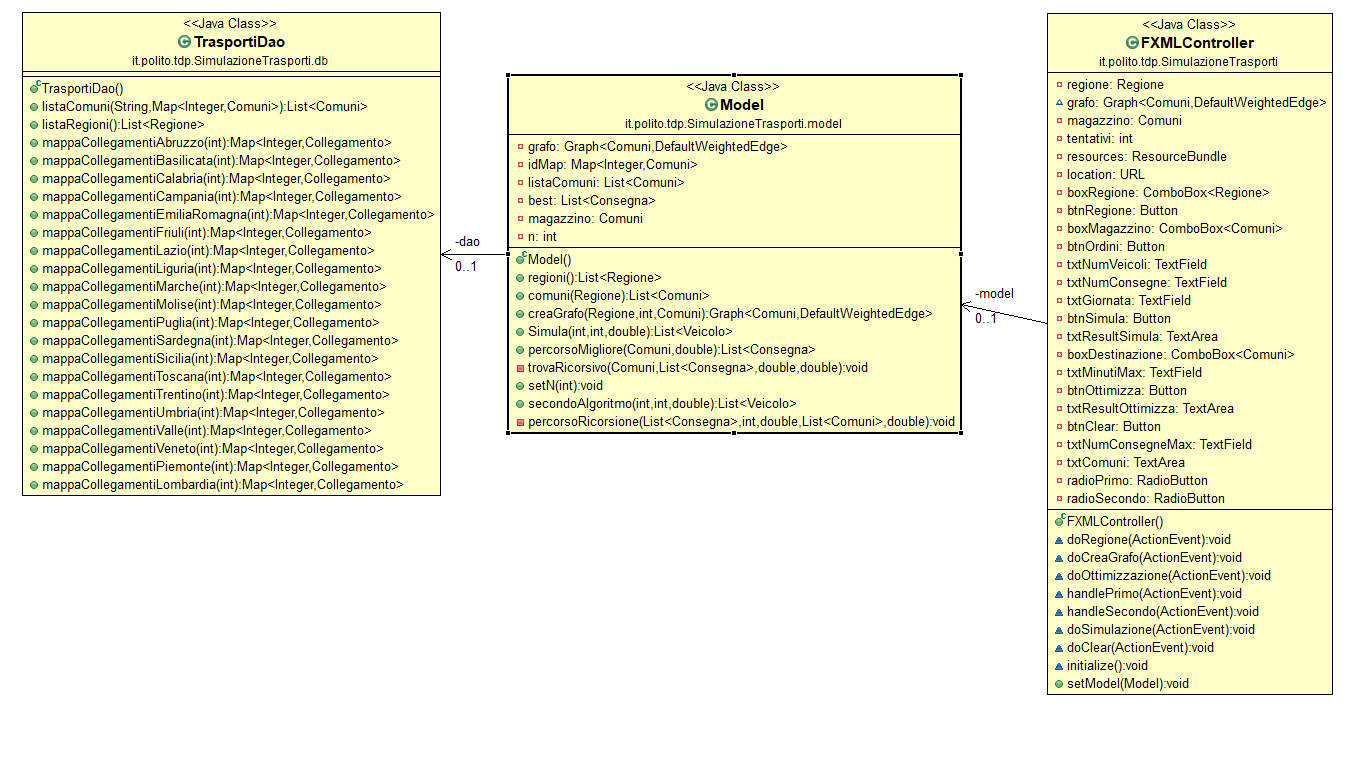
\includegraphics[width=0.8\paperwidth]{Images/DiagrammaUMLPrinc.png} 
\caption{Diagramma UML classi principali dei tre packages}  
\end{center}
\end{figure}

\begin{figure}[h]
\begin{center}
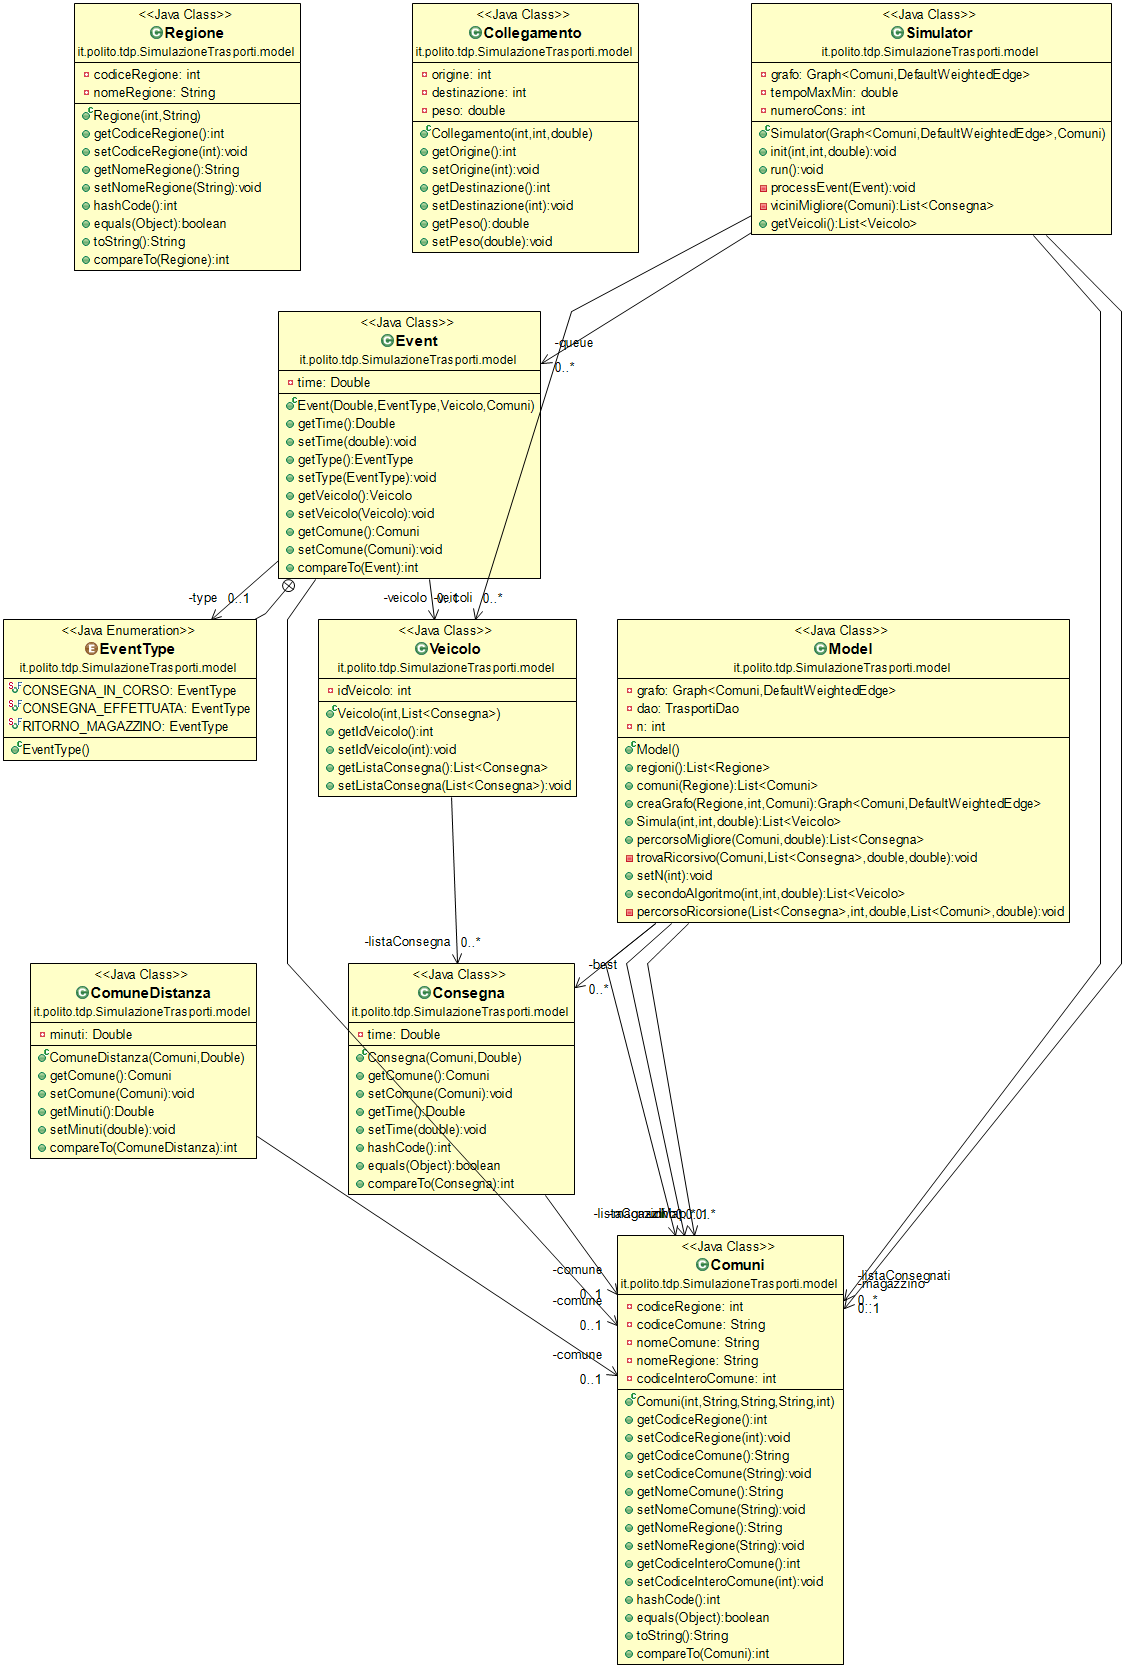
\includegraphics[width=0.6\paperwidth]{Images/Diagramma.png} 
\caption{Diagramma UML classi del model}  
\end{center}
\end{figure}
+

\chapter{Interfaccia dell'applicazione}


L'interfaccia utente dell'applicazione (Figura \ref{fig:interfaccia}) permette all'user di arrivare gradualmente alla simulazione
o ottimizzazione.\\
Scelta la regione e premuto il button \texttt{btnRegione} si accede alla fase successiva che richiede
magazzino principale e numero di ordini da simulare.\\
Dopo aver inserito i dati in input si accede all'ultima fase, ovvero il fine dell'applicazione: Simulazione
e Ottimizzazione.\\
Nella simulazione è importante decidere se utilizzare una simulazione bilanciata o non bilanciata.\\
La simulazione non bilanciata richiede l'inserimento di valori molto specifici per non sovraccaricare 
l'applicazione, perciò è richiesta molta attenzione nelle scelte da effettuare.\\
la simulazione bilanciata al contrario permette di inserire scenari molto più particolari e di osservare 
l'andamento dei veicoli in casi di ordini molto elevati.\\
La scelta della tipologia influenza anche il minutaggio impiegato per compiere il tragitto
da parte dei veicoli in caso essi vengano utilizzati al massimo delle loro capacità: la 
simulazione non bilanciata nella maggior parte dei casi ottiene risultati migliori in quanto si
preoccupa anche nel trovare il percorso che impiega meno tempo a parità di consegne.\\
Le due tipologie di simulazione sono strumenti di analisi differenti che se usati con accortezza
permettono di osservare scenari semi-realistici, perciò quando possibile conviene utilizzarli entrambi.\\
L'ottimizzazione del percorso richiede destinazione e minutaggio massimo e la sua velocità di esecuzione
è legata soprattutto al numero di ordini e minutaggio massimo.\\
In caso questi due numeri siano molto elevati è possibile che per giungere alla soluzione ci vogliano
diversi minuti.\\
Link al video dimostrativo: \href{https://youtu.be/MHyL_SAqDWc}{$https://youtu.be/MHyL_SAqDWc$}.
\begin{figure}[h]
\label{fig:interfaccia}
\begin{center}
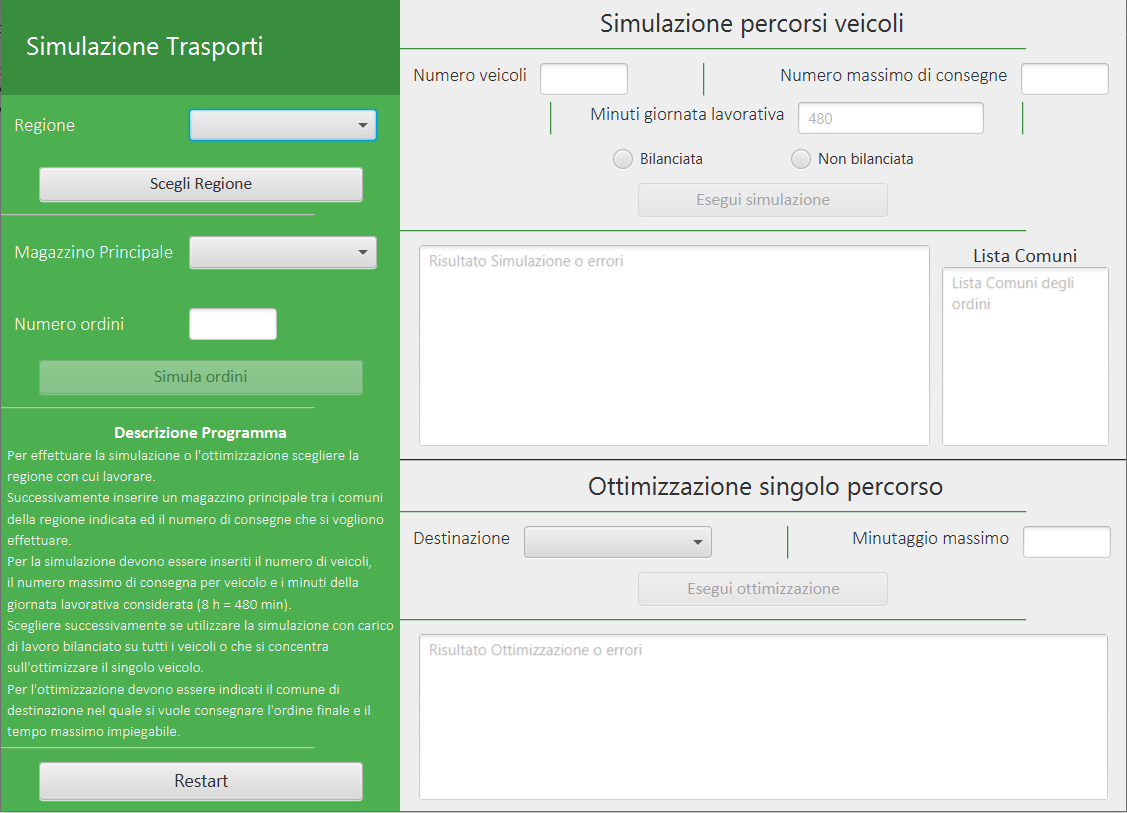
\includegraphics[width=0.8\paperwidth]{Images/Interfaccia.png} 
\caption{Interfaccia applicazione}
\end{center}
\end{figure}


\chapter{Risultati sperimentali ed esempi}
\section{Esempio 1}

\hrule
Regione: Lazio\\
Magazzino: Alatri\\
Numero Consegne: 15\\
\hrule
\begin{center}
\textbf{Lista Comuni}
\end{center}
Aquino\\
Campodimele\\
Colleferro\\
Colli sul Velino\\
Colonna\\
Marcetelli\\
Mentana\\
Morlupo\\
Patrica\\
Poggio Moiano\\
Rocca Santo Stefano\\
Rocca di Papa\\
Sant'Elia Fiumerapido\\
Tarano\\
Vico nel Lazio\\
\hrule
\begin{center}
\textbf{Input e Output Simulazione Bilanciata 1}
\end{center}
\textbf{Input}\\
Numero Veicoli: 3\\
Numero massimo di consegne: 5\\
Minuti giornata lavorativa: 480\\
\textbf{Output}\\
Numero ordini: 15\\

Id veicolo: 0	Numero consegne effettuate: 5\\
Comune: Vico nel Lazio	 Tempo (minuti): 10.96\\
Comune: Rocca Santo Stefano	 Tempo (minuti): 53.28\\
Comune: Mentana	 Tempo (minuti): 106.19\\
Comune: Poggio Moiano	 Tempo (minuti): 142.32999999999998\\
Comune: Marcetelli	 Tempo (minuti): 185.36999999999998\\
Ritorno al magazzino\\
Comune: Alatri	 Tempo (minuti): 267.15999999999997\\

Id veicolo: 1	Numero consegne effettuate: 5\\
Comune: Colleferro	 Tempo (minuti): 37.57\\
Comune: Colonna	 Tempo (minuti): 59.519999999999996\\
Comune: Rocca di Papa	 Tempo (minuti): 77.08\\
Comune: Morlupo	 Tempo (minuti): 123.81\\
Comune: Colli sul Velino	 Tempo (minuti): 188.55\\
Ritorno al magazzino\\
Comune: Alatri	 Tempo (minuti): 305.39\\

Id veicolo: 2	Numero consegne effettuate: 5\\
Comune: Patrica	 Tempo (minuti): 26.45\\
Comune: Aquino	 Tempo (minuti): 58.81\\
Comune: Sant'Elia Fiumerapido	 Tempo (minuti): 77.32000000000001\\
Comune: Campodimele	 Tempo (minuti): 122.9\\
Comune: Tarano	 Tempo (minuti): 231.89\\
Ritorno al magazzino\\
Comune: Alatri	 Tempo (minuti): 317.65\\

Numero consegne non effettuate: 0\\

\hrule
\begin{center}
\textbf{Input e Output Simulazione non Bilanciata 1}
\end{center}
\textbf{Input}\\
Numero Veicoli: 3\\
Numero massimo di consegne: 5\\
Minuti giornata lavorativa: 480\\
\textbf{Output}\\
Numero ordini: 15\\

Id veicolo: 0	Numero consegne effettuate: 5\\
Comune: Vico nel Lazio	 Tempo (minuti): 10.96\\
Comune: Patrica	 Tempo (minuti): 43.67000000000003\\
Comune: Colleferro	 Tempo (minuti): 73.71000000000004\\
Comune: Colonna	 Tempo (minuti): 95.66\\
Comune: Rocca di Papa	 Tempo (minuti): 113.21999999999997\\
Ritorno al magazzino\\
Comune: Alatri	 Tempo (minuti): 172.05999999999997\\

Id veicolo: 1	Numero consegne effettuate: 5\\
Comune: Rocca Santo Stefano	 Tempo (minuti): 44.94\\
Comune: Poggio Moiano	 Tempo (minuti): 99.27\\
Comune: Mentana	 Tempo (minuti): 135.41\\
Comune: Morlupo	 Tempo (minuti): 161.31000000000003\\
Comune: Tarano	 Tempo (minuti): 200.04\\
Ritorno al magazzino\\
Comune: Alatri	 Tempo (minuti): 285.8\\

Id veicolo: 2	Numero consegne effettuate: 5\\
Comune: Campodimele	 Tempo (minuti): 55.34\\
Comune: Aquino	 Tempo (minuti): 85.72\\
Comune: Sant'Elia Fiumerapido	 Tempo (minuti): 104.23\\
Comune: Marcetelli	 Tempo (minuti): 203.85000000000002\\
Comune: Colli sul Velino	 Tempo (minuti): 255.05\\
Ritorno al magazzino\\
Comune: Alatri	 Tempo (minuti): 371.89\\

Numero consegne non effettuate: 0\\
\hrule
\begin{center}
\textbf{Input e Output Ottimizzazione singolo percorso 1}
\end{center}
\textbf{Input}\\
Destinazione: Colli sul Velino\\
Minutaggio Massimo: 256\\
\textbf{Output}\\
Numero Consegne effettuate: 9\\
Comune: Alatri	 Tempo (minuti): 0.0\\
Comune: Vico nel Lazio	 Tempo (minuti): 10.96\\
Comune: Patrica	 Tempo (minuti): 43.67000000000003\\
Comune: Colleferro	 Tempo (minuti): 73.71000000000004\\
Comune: Colonna	 Tempo (minuti): 95.66\\
Comune: Rocca di Papa	 Tempo (minuti): 113.21999999999997\\
Comune: Mentana	 Tempo (minuti): 151.68\\
Comune: Morlupo	 Tempo (minuti): 177.58\\
Comune: Poggio Moiano	 Tempo (minuti): 215.19\\
Comune: Colli sul Velino	 Tempo (minuti): 253.95\\

\hrule
\begin{center}
\textbf{Input e Output Simulazione Bilanciata 2}
\end{center}
\textbf{Input}\\
Numero Veicoli: 3\\
Numero massimo di consegne: 9\\
Minuti giornata lavorativa: 480\\
\textbf{Output}\\
Numero ordini: 15\\

Id veicolo: 0	Numero consegne effettuate: 5\\
Comune: Vico nel Lazio	 Tempo (minuti): 10.96\\
Comune: Rocca Santo Stefano	 Tempo (minuti): 53.28\\
Comune: Mentana	 Tempo (minuti): 106.19\\
Comune: Poggio Moiano	 Tempo (minuti): 142.32999999999998\\
Comune: Marcetelli	 Tempo (minuti): 185.36999999999998\\
Ritorno al magazzino\\
Comune: Alatri	 Tempo (minuti): 267.15999999999997\\

Id veicolo: 1	Numero consegne effettuate: 5\\
Comune: Colleferro	 Tempo (minuti): 37.57\\
Comune: Colonna	 Tempo (minuti): 59.519999999999996\\
Comune: Rocca di Papa	 Tempo (minuti): 77.08\\
Comune: Morlupo	 Tempo (minuti): 123.81\\
Comune: Colli sul Velino	 Tempo (minuti): 188.55\\
Ritorno al magazzino\\
Comune: Alatri	 Tempo (minuti): 305.39\\

Id veicolo: 2	Numero consegne effettuate: 5\\
Comune: Patrica	 Tempo (minuti): 26.45\\
Comune: Aquino	 Tempo (minuti): 58.81\\
Comune: Sant'Elia Fiumerapido	 Tempo (minuti): 77.32000000000001\\
Comune: Campodimele	 Tempo (minuti): 122.9\\
Comune: Tarano	 Tempo (minuti): 231.89\\
Ritorno al magazzino\\
Comune: Alatri	 Tempo (minuti): 317.65\\

Numero consegne non effettuate: 0\\
\hrule
\begin{center}
\textbf{Input e Output Simulazione non Bilanciata 2}
\end{center}
\textbf{Input}\\
Numero Veicoli: 3\\
Numero massimo di consegne: 9\\
Minuti giornata lavorativa: 480\\
\textbf{Output}\\
Numero ordini: 15\\

Id veicolo: 0	Numero consegne effettuate: 9\\
Comune: Vico nel Lazio	 Tempo (minuti): 10.96\\
Comune: Aquino	 Tempo (minuti): 55.06000000000001\\
Comune: Sant'Elia Fiumerapido	 Tempo (minuti): 73.57000000000001\\
Comune: Patrica	 Tempo (minuti): 118.07999999999998\\
Comune: Colleferro	 Tempo (minuti): 148.11999999999998\\
Comune: Colonna	 Tempo (minuti): 170.06999999999994\\
Comune: Rocca di Papa	 Tempo (minuti): 187.62999999999994\\
Comune: Mentana	 Tempo (minuti): 226.08999999999995\\
Comune: Morlupo	 Tempo (minuti): 251.98999999999998\\
Ritorno al magazzino\\
Comune: Alatri	 Tempo (minuti): 331.99\\

Id veicolo: 1	Numero consegne effettuate: 6\\
Comune: Campodimele	 Tempo (minuti): 55.34\\
Comune: Rocca Santo Stefano	 Tempo (minuti): 141.88000000000005\\
Comune: Marcetelli	 Tempo (minuti): 195.63000000000005\\
Comune: Poggio Moiano	 Tempo (minuti): 238.67000000000004\\
Comune: Colli sul Velino	 Tempo (minuti): 277.43000000000006\\
Comune: Tarano	 Tempo (minuti): 324.59000000000003\\
Ritorno al magazzino\\
Comune: Alatri	 Tempo (minuti): 410.35\\

Id veicolo: 2	Numero consegne effettuate: 0\\

Numero consegne non effettuate: 0\\
\hrule
\subsection*{Valutazioni}
Nell'esempio 1 è stata effettuata una simulazione bilanciata, non bilanciata ed
ottimizzazione di uno scenario svolto nella regione Lazio, magazzino ad Alatri e con numero di ordini uguale a 15.\\
Viene prima analizzata la simulazione bilanciata (\texttt{Input e Output Simulazione Bilanciata 1}) che è effettuata con 3 veicoli, numero massimo
di consegne da effettuare 5 in 480 minuti e come previsto si ottengono 3 percorsi con 5 consegne ciascuna.\\
Data la grandezza della regione sono state effettuate tutte le consegne e i veicoli tornano al magazzino
all' incirca nello stesso range di 60 minuti, perciò in questo caso il lavoro risulta bilanciato.\\
Per osservare altri risultati utilizziamo la Simulazione non bilanciata (\texttt{Input e Output Simulazione non Bilanciata 1}) e notiamo come anche nel secondo caso
i percorsi sono formati da 5 consegne ciascuna e nessuna consegna non effettuata.\\
Si nota però una leggera discrepanza nel ritorno al magazzino, difatti il primo mezzo ritorna dopo 
172.05 minuti mentre l'ultimo dopo 371.89 minuti.\\
Ciò permette di dire che risulta migliore la simulazione non bilanciata poiché il tempo
totale impiegato dai mezzi per tornare a magazzino è minore della Simulazione bilanciata.\\
Perciò a seconda di come vuole essere impostato lo scenario scegliamo il sistema di percorsi ottenuti
adatti al caso.\\
A questo punto si pone un problema: il percorso del veicolo con ID:2 è ottimizzato? Per come è impostato l'algoritmo
infatti viene ottimizzato prima il primo percorso e poi quelli successivi.\\
Allora si può sfruttare l'ottimizzazione (\texttt{Input e Output Ottimizzazione singolo percorso}): in 256 minuti e con destinazione Colli sul Velino (ultima
consegna veicolo ID:2) quante consegne massime si possono effettuare?
La risposta è 9, perciò si nota come l'ultimo veicolo non sia affatto ottimizzato.\\
Per questo motivo si può effettuare un altro tentativo con scenario differente: Simulazione 
con 9 massime consegne per veicolo al posto di 5.\\
La Simulazione bilanciata (\texttt{Input e Output Simulazione Bilanciata 2}) ottiene lo stesso risultato precedentemente ottenuto in quanto
dà ai veicoli lo stesso carico di lavoro.\\
La simulazione non bilanciata (\texttt{Input e Output Simulazione non Bilanciata 2}) invece cambia notevolmente: il veicolo con ID:0 effettuata 9 consegne
e torna nel magazzino in 331.99 minuti\footnote{Il veicolo nella simulazione raggiunge l'ultima consegna prima di quella ottenuta con l'ottimizzazione
in quanto non ha il vincolo della destinazione}, il veicolo con ID:1 effettua 6 consegne e il veicolo con 
ID:3 nemmeno una.\\
In questo caso si è riusciti con mezzi più grandi a diminuire il numero di veicoli necessari nonostante
precedentemente potesse sembrare che i mezzi fossero saturi.\\
Quindi se a disposizione di veicoli con capienza diversa e nel caso in cui si voglia sfruttare 
ogni minuto a disposizione la simulazione non bilanciata offre la soluzione migliore, mentre in 
altro caso la bilanciata risulta la soluzione più accettabile.\\

\section{Esempio 2}
\hrule
Regione: Emilia Romagna\\
Magazzino: Alseno\\
Numero Consegne: 15\\
\hrule
\begin{center}
\textbf{Input e Output Simulazione Bilanciata 3}
\end{center}
\textbf{Input}\\
Numero Veicoli: 3\\
Numero massimo di consegne: 5\\
Minuti giornata lavorativa: 480\\
\textbf{Output}\\
Numero ordini: 15\\

Id veicolo: 0	Numero consegne effettuate: 4\\
Comune: Pellegrino Parmense	 Tempo (minuti): 29.02\\
Comune: Concordia sulla Secchia	 Tempo (minuti): 119.14999999999999\\
Comune: Montese	 Tempo (minuti): 214.89999999999998\\
Comune: Castrocaro Terme e Terra del Sole	 Tempo (minuti): 335.65999999999997\\
Ritorno al magazzino\\
Comune: Alseno	 Tempo (minuti): 474.91999999999996\\

Id veicolo: 1	Numero consegne effettuate: 5\\
Comune: Bologna	 Tempo (minuti): 74.41\\
Comune: Voghiera	 Tempo (minuti): 108.16999999999999\\
Comune: Lagosanto	 Tempo (minuti): 134.0\\
Comune: Alfonsine	 Tempo (minuti): 185.96\\
Comune: Brisighella	 Tempo (minuti): 226.77\\
Ritorno al magazzino\\
Comune: Alseno	 Tempo (minuti): 355.49\\

Id veicolo: 2	Numero consegne effettuate: 4\\
Comune: Bore	 Tempo (minuti): 32.7\\
Comune: Vergato	 Tempo (minuti): 153.94\\
Comune: Lugo	 Tempo (minuti): 233.47\\
Comune: Galeata	 Tempo (minuti): 302.75\\
Ritorno al magazzino\\
Comune: Alseno	 Tempo (minuti): 473.22\\

Numero consegne non effettuate: 2\\
\hrule
\subsection*{Valutazioni}
Nell'esempio considerato è stata effettuata una simulazione bilanciata
in Emilia-Romagna, magazzino ad Alseno e 15 ordini effettuati.\\
La simulazione bilanciata (\texttt{Input e Output Simulazione Bilanciata 3}) è stata effettuata con 3 veicoli e con 5 massime consegne per veicolo.\\
L'output ottenuto mostra come non siano state effettuate 2 consegne nonostante la richiesta e i mezzi
siano simili a quelli della regione Lazio svolta in precedenza (\texttt{Output Simulazione Bilanciata 1}).\\
In questo caso infatti la variabile legata alla grandezza della regione ha giocato un ruolo importante
ed è chiaro osservando il ritorno al magazzino dei mezzi, più o meno intorno al minuto 480.\\
Perciò nella scelta del numero di veicoli e del numero massimo di consegne è necessario tenere conto
anche della regione considerata.\\


\chapter{Valutazioni finali e conclusioni}
L'applicazione sviluppata riesce nell'intento di costituire uno strumento utile all'analisi dei
trasporti su gomma per una qualsiasi azienda.\\
Gli algoritmi sviluppati sono in grado di sopperire l'uno alla mancanza dell'altro e di aiutare
l'utente a scegliere una soluzione accettabile una volta scelte le variabili.\\
Analizzando gli obiettivi posti in fase di progetto ed elencati nel Capitolo \ref{cap:Descrizione} si nota come essi
siano o direttamente o indirettamente soddisfatti.
\begin{description}
\item[Efficienza dei processi] L'utilizzo delle varie opzioni presenti nell'applicazione serve ad
aumentare la qualità del percorso di ogni singolo veicolo.
\item[Qualità delle infrastrutture relative al commercio e al trasporto] Per qualità in questo caso
si intende capienza massima di ogni veicolo e tramite l'applicazione è possibile valutare quale
sia la migliore quantità per permettere un utilizzo adeguato e funzionale.
\item[Capacità di rintracciare e seguire le spedizioni] Tale obiettivo è stato parzialmente considerato
in quanto necessario per valutare il tragitto del veicolo.
\item[Frequenza con la quale le spedizioni raggiungono i destinatari entro i tempi]  Questo obiettivo viene direttamente sviluppato dall'utente ed è legato al fatto che
si preferisce effettuare tutte le consegne rispetto a sfruttare al massimo ogni mezzo. \\
Infatti l'utente riformulando più volte lo scenario con variabili costanti deve sempre ottenere
\texttt{numero di consegne non effettuate}=0.
\end{description}
Tuttavia i limiti dell'applicazione sono tanti e come già elencati nel Capitolo \ref{Cap:DescrizioneStrutture}, Sezione \ref{Sec:Algoritmi} sono numerosi
i miglioramenti che possono essere svolti.\\
Non tenendo conto del magazzino e delle risorse umane l'applicazione si concentra solo nel creare
percorsi adeguati alle caratteristiche volute.\\
Un'altra criticità è legata al tempo impiegato dall'applicazione per svolgere le operazioni.\\
In particolar modo la simulazione non bilanciata e l'ottimizzazione sfruttando la ricorsione richiedono
una complessità computazionale non indifferente e perciò richiedono l'utilizzo di variabili contenute.\\
Per un miglioramento futuro dell'applicazione perciò è consigliato partire dalla velocità di esecuzione
dei due algoritmi, magari imponendo più vincoli intermedi nella ricerca del risultato migliore.


\clearpage
\null

\vspace{\fill}
\begin{center}
\begin{figure}[h]
\begin{center}

\includegraphics[width=0.25\textwidth]{Images/License.png} 
\end{center}
\end{figure}
Quest’opera è distribuita con licenza Creative Commons «Attribuzione – Non
commerciale – Condividi allo stesso modo 4.0 Internazionale».\\
Copia della licenza consultabile al sito web:
\href{https://creativecommons.org/licenses/by-nc-sa/4.0}{https://creativecommons.org/licenses/by-nc-sa/4.0}.
\end{center}

\clearpage

\end{document}